\documentclass[6pt]{article}
\usepackage[utf8]{inputenc}
\usepackage{graphicx}
\usepackage[T1]{fontenc}
\usepackage{tgpagella}
\usepackage{fancyhdr}
\pagestyle{fancy}
\fancyhf{}
\renewcommand{\headrulewidth}{0pt} 
\rhead{\scriptsize{\textbf{An Approach to Intelligent Interactive Social Network Geo-Mapping}}}

\begin{document}
\title{\bf \Large An Approach to Intelligent Interactive Social Network Geo-Mapping \normalsize \rm}

\author{Anton Benčič, Márius Šajgalík, Michal Barla, Mária Bieliková}
\date{}
\maketitle
\begin{center}
Slovak University of Technology in Bratislava\\
Faculty of Informatics and Information Technologies\\
Ilkovičova 3, 842 16 Bratislava, Slovakia\\
{name.surname}@stuba.sk\\
\end{center}



\bf \abstractname \rm { Map-based visualization of different kinds of information, which can be geo-coded to a particular location, becomes more and more popular, as it is very well accepted and understood by end-users. However, a simple map interface is not enough if we aim to provide information about objects coming from vast and dynamic information spaces such as the Web or social networks are. In this paper, we propose a novel method for intelligent visualization of generic objects within a map interface called IntelliView, based on an extensive evaluation and ranking of objects including both content and collaborative-based approaches. We describe the method implementation in a web-based application called Present, which is aimed at recycling items in social networks together with an experiment aimed at evaluation of proposed approach.}
 
\section{Introduction and Related Work}
Intelligent presentation of data and information on the Web, including personalization is becoming crucial as the amount of available information increases in an incredible pace while the information is getting inter-connected in various different ways. It is becoming harder and harder to navigate in such a tangle of information resources of various kinds, origin and quality.

Special kind of information, which is gaining popularity nowadays, is information coming from social networks. Visualization of social networks is often realized in a form of complicated graphs that are hard to read and navigate in. Other approach is to use text interfaces to provide information about events happening within a social network. Neither of these approaches can keep pace with dynamics of social network and does not scale well as the size of the social network grows as well as the amount of information within it.

Most of the well-known approaches to social network visualization are not targeted at end-users, but rather on researchers or analysts, providing them with a quick overview of a social network and means for further statistical analysis and sociological research \cite{yang2008visual}.




An example of a system, which is devoted to be used by end-users, is Viszter \cite{heer2005vizster}. It visualizes a social network in a force-directed network layout. It focuses on using different visualization techniques to improve the navigation and search experience, but does not include any kind of content filtering or personalization, which would help to reduce the size of displayed network.

We decided to tackle the issue by realizing an intelligent map interface support for social networks visualization. A map, forming a basis of the visualization is a well known concept providing a basic level of information space partitioning based on geographical location. Location is often basic attribute of people or things involved in the social network. Another important partitioning is obtained by intelligent evaluation of social network, which partition the whole graph into several layers of abstraction and thus preventing the information overload problem.

There are many production-grade solutions based on map visualization, usually built on top of big online map services providers such as Google Maps or Microsoft Bing Maps. The system Geotracker \cite{chen2007geotracker} is interesting from our point of view, as it, apart from using the map interface to visualize geotagged RSS content, provides also a possibility to visualize development of the information space over time, which is similar to our idea of RealView described in this paper. Moreover, it contains basic user’s interests model mapped to content categories, which is used for the personalization of the presentation layer.

In order to capture the dynamics of social networks, we also visualize important events and interactions. These are fully adapted to a user, to give him an overview of what happened since his last visit and to provide him with real-time updates as they happen.

Every visualization method obviously aims at presenting the most relevant content for a particular user. In the case when there are too many objects, which cannot be presented efficiently all at the same time, the first step that has to be exploited in one way or another is the content filtering. The first filtering that our approach called IntelliView performs is on a basis of the currently visible region of the map. However, this is far away from being enough, as the extent of a visible map can and by experience contains more content (objects) that can be presented at a time.

Because of this, our IntelliView makes another use of content filtering in a two-step process: (i) object evaluation and (ii) content presentation (visualization).

This paper is structured as follows. In first two sections we describe two basic steps of the proposed method for visualization: object evaluation \ref{3} and concept visualization \ref{4}. Section 5 is devoted to the evaluation of proposed method. Finally, we draw our conclusions.

\footnotetext{The best-known tools for visualizing and analyzing social networks are UCINET (http://www.analytictech.com/ucinet/) and PAJEK (http://pajek.imfm.si/).}


\section{Object Evaluation}
The main issue of any kind of presentation-layer preprocessing is that if we want to get more accurate results, we need more data to collect and need to spend more time per object for its evaluation. If we are using a lengthy evaluation method in a real world (i.e. the Web) environment with many objects to evaluate, this can be a problem as the users are willing to wait only a very limited time for the site or application to respond and if it does not, the user most often gives up.

An often used technique for overcoming the time problem is caching or pre-computing. Caching can help users speed up their consequent requests and is most useful in an environment where users follow a use pattern or tend to repeat their use-cases over a period of time. However, if there is large diversity in user behavior or the evaluation depends on time-varying parameters, the stored results become obsolete very quickly and the whole concept of caching fails. The technique of pre-computing has the same purpose and problems as caching with the difference that pre-computing is used for more complex computations that change even less often and their results are used for processing of each request.

Because our method for intelligent visualization of generic objects within a map interface needs to work with large sets of objects and present only a small portion of them at a time, we need more complex and thus time consuming computations to perform on every object. However, due to the aforementioned problem of computation and response times, we were forced to move some portions of the process into pre-computations stage.

Our object evaluation algorithm has both content-based and collaborative components. 
The final value for an object is assigned as follows:
 
$$k=c_ok_o+c_pk_p+c_ck_c $$

where $c_o$, $c_p$ and $c_c$ are constant coefficients that together sum up to one,
\begin{itemize}
\item $k_o$ represents the index of general object significance,
\item $k_p$ is the index of personal object significance and
\item $k_c$ is the index of collaborative object significance.
\end{itemize}

The first two indexes are computed on request basis as they are content-based and may change more swiftly while the third, collaborative index is pre-computed on daily basis as its nature is much less dynamic.

\subsection{General Object Significance}

General object significance component tells how significant an object is to a random user without considering any personalization. It is computed as a sum of three subcomponents:

\begin{itemize}
\item Explicit feedback for the object coming from all system users.
\item Object's lifetime within the system, with a negative correlation to object's significance (older objects are less significant than more recent ones).
\item Category significance, assigned by an expert.
\end{itemize}

The three given parameters are put together in an equation:

$$k_o=c_{sup}d(\#of~supports)+c_{cat}d(cat.sig.)-c_{tim}d(time)$$

The $c_{sup}$, $c_{cat}$ and $c_{tim}$ are coefficients that set the significance of single components and that sum up to one and determine the weight of aforementioned subcomponents into the overall significance. The coefficients are set by a domain expert, but can be also discovered dynamically. In our representative implementation we started by manually estimating these coefficients according to the evaluation of a few representative test objects and subsequently these values were gradually fine-tuned dynamically and per-user by evaluating user’s behavior and interaction with objects within the system as mentioned.

The equation also features a distribution function d that is an integral part of the content-based part of the evaluation algorithm. Its purpose is to distribute the outputs between zero and one in a way that the difference is most significant around the evaluated set’s median. The distribution function is given by the following equation:

\large $$d(x)=\frac{tan^{-1}\Big(\frac{x}{\frac{median(X)}{a}}-a\Big)+tan^{-1}a}{\frac{PI}{2}+tan^{-1}a}$$ \normalsize

The equation takes besides the input value two more parameters, which are constant throughout one iteration on a set of objects. The median(X) is a median value of the set of object parameters and the value a defines how sharp will be the edge between relaxed parts of the function and the steep part. The difference is shown in Figure 1, where both have the median of 100, the function in Figure 1a has a=pi/2 and the function in Figure 1b has a=4pi.

\begin{figure}[h]
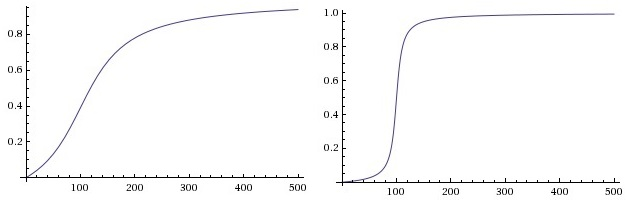
\includegraphics[width=\textwidth]{images/fig.jpg}
\caption{Distribution function with (a) a=pi/2, (b) a=4pi.}
\end{figure}

\subsection{Personal Object Significance}
The purpose of the personal object significance value is to encourage objects that the user might have interest in. The equation is as follows:

$$k_p=c_{cat} d(category~rank)+c_{kword} d(top~keyword~rank) $$

The $c_{cat}$, $c{kword}$ and $c_{sup}$ are again coefficients of component significances that sum up to one. These coefficients can be set in a similar manner as in general object significance calculation and in our representative implementation we set them in the selfsame way. The category rank is a number derived from an ordered set of the user’s N most popular categories.


It is expressed as:

$$category~rank=\frac{N-[category~position]+1}{N}$$


The equation shows that the rank is determined by the category’s position in the ordered set. The set always stores N most popular categories, where N is chosen by the environment’s properties such as number of categories, number of users storage capacity and computation power, because these numbers need to be stored in a persistent storage and storing large number of categories for a large number of users would not be sustainable. The category’s position is determined by the user’s interest value that is raised every time user gives a positive implicit or explicit feedback to an object from that category while decreasing this value for all other categories. Once a category’s value for a given user drops below a set threshold value, it is removed from the ordered set and a new category that the user developed an interest in recently can be stored. If a category is not contained within the set, its rank for the given user will be zero.

The top keyword rank works in a similar way to the category rank with the difference that it takes the top keyword contained within both object name, description, etc. and the table of top N keywords.

\subsection{Collaborative Object Significance}

Collaborative component of the evaluation function takes into account interests and activities not only of the user that the evaluation is meant for, but also users similar to him. Similar user is a fuser who has an interest in the same object categories and/or searches for the same keywords. As we are working with graph-like structures, we can take advantage of graph-based algorithms such as spreading activation \cite{berthold2008supporting}, HITS \cite{mining2006exploring} or PageRank \cite{page1999pagerank} to find and rank similar and related users or objects.

When we find such a user, we assume that objects of his interest might be of interest to the current user as well. The evaluation is done in a similar way as the previous two components taking into account the level of similarity of the two users and the trustfulness of the similar user given by his rating.

\section{Content Visualization}
\label{3}

 

Due to enormous number of objects to be displayed, IntelliView has to choose only a small subset of them in order to maintain a lucid view. To accomplish this, objects are sorted by priority – a number that comes from the object evaluation described in the section 2. Prioritization is reflected by the most common visualization techniques that can be found in Bing Maps, Google maps or in a well-known ESRI’s geographic information system (GIS) software products.

With the list of objects sorted by priority, IntelliView aims to achieve the following basic goals:
\begin{itemize}
\item{displaying as much information as possible,}
\item{displaying objects with higher priority first,}
\item{illustrating the density of objects,}
\item{maintaining a simple view.}
\end{itemize}



We proposed two main methods for displaying objects, each of them with its own pros and cons. First, probably the most intuitive, method is depicted in Figure 2. There we can see a personalized view of Central Europe. Despite such a large area there in Slovakia emerges the local collection for people affected by the earthquake in Haiti. This is because of extensive donation of items made there by the user, his friends in social networks and other local users within that location. This first method has shown to be more successful and attractive to users than the second one.

In this method, objects are sorted and iterated over by their priority. For every object being iterated we check, whether there is or is not a collision with other objects, which are already displayed. If there is no collision, the object is displayed. If there is a collision, the object is considered to be displayed with less importance and in order not to overlay those already displayed (which have evidently higher priority), its size is reduced and opacity decreased. Ordered by importance, the objects are grouped into several levels of importance. Visually, displayed items differ based on the level, which they are included in.

To maintain lucid view, object distribution is pushed to the last level, which is not displayed. Thus, visual differences among levels can be less significant. Presence of hidden items in the last level is represented by background color of appropriate topmost item. In this manner, density can be viewed as well. Advantage of this method is in accurate projection of item location, but considering priority order, items in higher levels can have lower priority than those in lower levels.

The second method tries to achieve greater accuracy of displaying priority by dividing the whole viewport into a grid and considering items isolated, individually in each cell. Thus, each cell has its own representative, which is dominating in the center of this cell. Items in lower levels of importance are displayed similarly as in preceding method around cell's representative. While having improved accuracy of priority order depiction, this method has also better performance in calculation following principles of divide and conquer.

However, in this case, location of item cannot be determined due to an error caused by the centralization within cell. The goal of centralization is to avoid collision
problems on neighboring cell's bounds. As a positive side effect, due to uniform distribution of items on the map, this view is symmetric and more readable, but it may appear a bit artificial because of that. Finally, we abandoned this method due to its unattractiveness for users.

\begin{figure}[h]
\centering
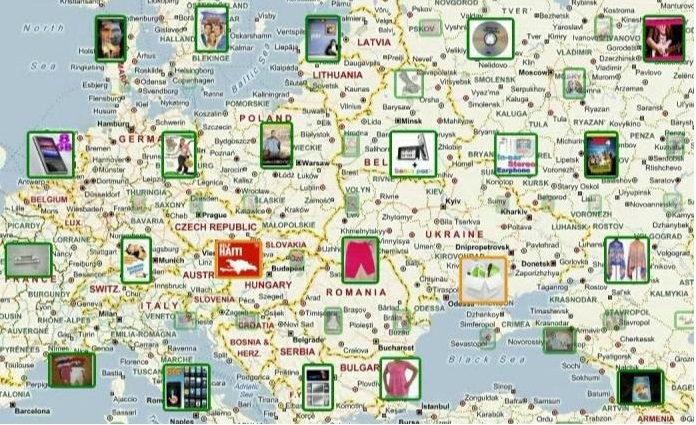
\includegraphics[width=0.8\textwidth]{images/fig3.jpg}
\caption{Personalized visualization of IntelliView}
\end{figure}

\section{Real-time Visualization of Social Network Dynamics}
\label{4}
If we want the users to understand the dynamics of the information space, which is being visualized, we need to clearly present the (relevant) transitions between various states within the information space. The RealView algorithm processes actions that other users perform within the viewing area and displays them as animations on the map.

The algorithm could just show all or at least majority of the actions, but it would not be practical for a couple of reasons. First of all with rising number of actions, the traffic increases as well. Second, the purpose of this dynamic view is to bring the user activity to encourage him to be active as well, but overwhelming him with animations would rather be counterproductive. That is why we implemented a filtering system, whose purpose is to select which actions will be delivered to the individual users.

The decision process is time sensitive and is based on a modified version of the relevancy system that is used in IntelliView. The time sensitivity means that despite of not showing all of the actions in the viewing area, the algorithm still has to be aware of the rate at which the actions happen. When implementing the mentioned features, we cannot work in true real-time. The basic idea is to stack the animations in a list, putting a delay interval between them that reflects the activity rate.

We briefly introduce two specific implementations of this concept. The first algorithm maintains an ordered list of actions and the number of actions from the last animation. Then every time a given number of actions are processed, it picks the first one and displays its animation.
The ordering is performed in a following way:

\begin{itemize}
\item{when an action is intercepted, its relevancy value is calculated,}
\item{all actions with lower relevancy are dismissed from the list,}
\item{the processed action is added to the end of the list.}
\end{itemize}
This ensures that the first action in the list has always the highest relevancy and that we keep all consequent animations.

The second algorithm is a simplification of the first one. It stores only one, most relevant action and the number of actions from the last animation. Then every time a given number of actions were processed it displays the stored animation.

\section{Evaluation}
In order to evaluate our approach to intelligent information visualization, we developed a web-based system called Present, which aims to help preventing precious nature resources by supporting re-use of ordinary goods and items instead of their endless production (see Figure 3). This is done by providing people with efficient means for donating or lending items, which are functional, but not used any more, and on the other side for requesting such donations or lendings.

\begin{figure}[ht]
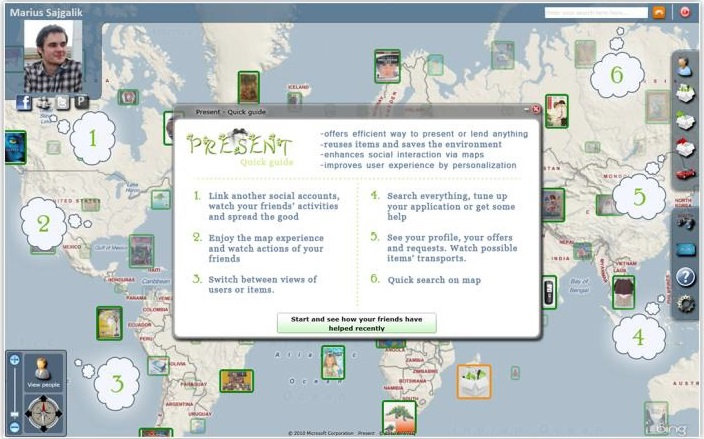
\includegraphics[width=\textwidth]{images/fig4.jpg}
\caption{Present – introduction screen.}
\end{figure}

Present is strongly connected to existing social networks such as Facebook, which play a crucial role not only in spreading the information about the system to new users, but also in providing a continuous motivation to use the system. This is achieved also by posting automatic updates to user's wall including photos of things he has provided, things he has borrowed or lent, events he has done, etc. and regular updates with user statistics, social impact information and posts about successful stories.

In addition to common statistics of the user activity, there are statistics provided by user geographical location. They include amount of welfare done in his location, statistics of users from his neighborhood and especially comparison with neighboring regions and countries. This indirectly leads to geo-competition and bigger interest in our system.

In order to evaluate the proposed approach, we filled the Present with artificial testing data about people, their items, donations and borrowings. The instances, albeit being generated artificially, were not completely random. We employed genetic algorithm-like approach to perform crossovers between instances, so that a new instance would contain meaningful and credible attributes.

This way we were able to generate 2.7 million of virtual users placed on a map by following population density on our Earth. The system was running smoothly on an average personal computer in the role of a server even with such a great number of objects to be processed and displayed, which proves that the solution can be deployed in real-world conditions. Moreover, the real-world deployment could take advantage of cloud computing to distribute and handle the load.

Apart from basic evaluation of technical viability of the approach, we conducted a user-study with 25 volunteers, which were asked to use the system and provide us with feedback by filling-in a questionnaire. The majority of participants (76) were attracted by the map interface immediately and 60 of them expressed that they were feeling comfortable when navigating on the map and found the layout of objects on the top of the map very well arranged (see \ref{fig4}).
\begin{figure}[ht]
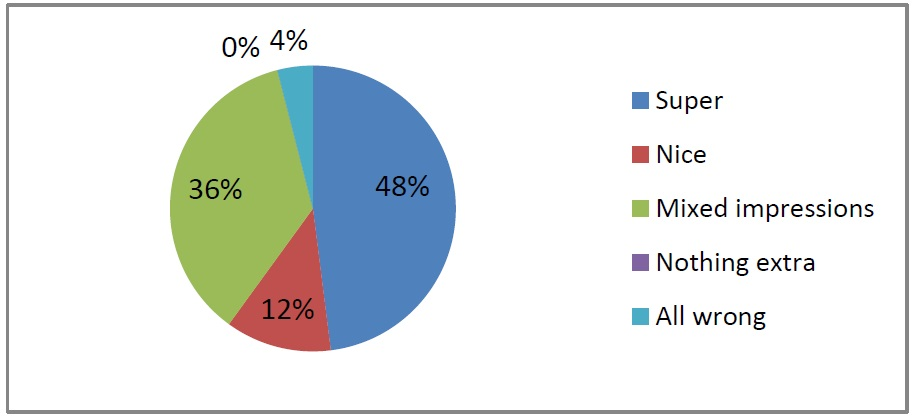
\includegraphics[width=\textwidth]{images/fig5.jpg}
\caption{Opinions of participants on the items and actions visualization on the screen and navigation among them.}
\label{fig4}
\end{figure}

\section{Conclusion}
In this paper we presented a novel approach to visualization of large amounts of geo-coded and dynamic information, which can be nowadays found in social networks. Social data are getting more and more interest, as the Social Web spreads outside the environment of the isolated "social" applications and becomes a ubiquitous part of the ordinary Web. Traditional web-based information systems must take this into account and incorporate intelligent approaches in order to provide their users with the most relevant results while prevent information overload.

This is what we aimed at by our approach to information space visualization based on the intelligent map interface, which takes into account usage data of an individual as well as all users of system to determine user interests expressing what kind of content is relevant for the user and layout the content on the top of the map appropriately.

We evaluated the approach on the web-based system Present, which was filled with non-trivial amount of data and evaluated within a user study. The results showed that the chosen visualization paradigm combined with the intelligent processing behind it provides an efficient means for personalized navigation within vast information spaces.

\begin{description}
 \item  \bf Acknowledgement. \rm This work was partially supported by the grants VG1/0508/09, APVV-0208-10 and it is the partial result of the Research \& Development Operational Programme for the project Support of Center of Excellence for Smart Technologies, Systems and Services II, ITMS 26240120029, co-funded by the ERDF.
\end{description}

\bibliographystyle{plain}
\bibliography{zdroje}


\end{document}
